\documentclass[twoside]{book}

% Packages required by doxygen
\usepackage{calc}
\usepackage{doxygen}
\usepackage{graphicx}
\usepackage[utf8]{inputenc}
\usepackage{makeidx}
\usepackage{multicol}
\usepackage{multirow}
\usepackage{textcomp}
\usepackage[table]{xcolor}

% Font selection
\usepackage[T1]{fontenc}
\usepackage{mathptmx}
\usepackage[scaled=.90]{helvet}
\usepackage{courier}
\usepackage{amssymb}
\usepackage{sectsty}
\renewcommand{\familydefault}{\sfdefault}
\allsectionsfont{%
  \fontseries{bc}\selectfont%
  \color{darkgray}%
}
\renewcommand{\DoxyLabelFont}{%
  \fontseries{bc}\selectfont%
  \color{darkgray}%
}

% Page & text layout
\usepackage{geometry}
\geometry{%
  a4paper,%
  top=2.5cm,%
  bottom=2.5cm,%
  left=2.5cm,%
  right=2.5cm%
}
\tolerance=750
\hfuzz=15pt
\hbadness=750
\setlength{\emergencystretch}{15pt}
\setlength{\parindent}{0cm}
\setlength{\parskip}{0.2cm}
\makeatletter
\renewcommand{\paragraph}{%
  \@startsection{paragraph}{4}{0ex}{-1.0ex}{1.0ex}{%
    \normalfont\normalsize\bfseries\SS@parafont%
  }%
}
\renewcommand{\subparagraph}{%
  \@startsection{subparagraph}{5}{0ex}{-1.0ex}{1.0ex}{%
    \normalfont\normalsize\bfseries\SS@subparafont%
  }%
}
\makeatother

% Headers & footers
\usepackage{fancyhdr}
\pagestyle{fancyplain}
\fancyhead[LE]{\fancyplain{}{\bfseries\thepage}}
\fancyhead[CE]{\fancyplain{}{}}
\fancyhead[RE]{\fancyplain{}{\bfseries\leftmark}}
\fancyhead[LO]{\fancyplain{}{\bfseries\rightmark}}
\fancyhead[CO]{\fancyplain{}{}}
\fancyhead[RO]{\fancyplain{}{\bfseries\thepage}}
\fancyfoot[LE]{\fancyplain{}{}}
\fancyfoot[CE]{\fancyplain{}{}}
\fancyfoot[RE]{\fancyplain{}{\bfseries\scriptsize Generated on Tue Sep 25 2018 12\-:55\-:43 for editor by Doxygen }}
\fancyfoot[LO]{\fancyplain{}{\bfseries\scriptsize Generated on Tue Sep 25 2018 12\-:55\-:43 for editor by Doxygen }}
\fancyfoot[CO]{\fancyplain{}{}}
\fancyfoot[RO]{\fancyplain{}{}}
\renewcommand{\footrulewidth}{0.4pt}
\renewcommand{\chaptermark}[1]{%
  \markboth{#1}{}%
}
\renewcommand{\sectionmark}[1]{%
  \markright{\thesection\ #1}%
}

% Indices & bibliography
\usepackage{natbib}
\usepackage[titles]{tocloft}
\setcounter{tocdepth}{3}
\setcounter{secnumdepth}{5}
\makeindex

% Hyperlinks (required, but should be loaded last)
\usepackage{ifpdf}
\ifpdf
  \usepackage[pdftex,pagebackref=true]{hyperref}
\else
  \usepackage[ps2pdf,pagebackref=true]{hyperref}
\fi
\hypersetup{%
  colorlinks=true,%
  linkcolor=blue,%
  citecolor=blue,%
  unicode%
}

% Custom commands
\newcommand{\clearemptydoublepage}{%
  \newpage{\pagestyle{empty}\cleardoublepage}%
}


%===== C O N T E N T S =====

\begin{document}

% Titlepage & ToC
\hypersetup{pageanchor=false}
\pagenumbering{roman}
\begin{titlepage}
\vspace*{7cm}
\begin{center}%
{\Large editor }\\
\vspace*{1cm}
{\large Generated by Doxygen 1.8.6}\\
\vspace*{0.5cm}
{\small Tue Sep 25 2018 12:55:43}\\
\end{center}
\end{titlepage}
\clearemptydoublepage
\tableofcontents
\clearemptydoublepage
\pagenumbering{arabic}
\hypersetup{pageanchor=true}

%--- Begin generated contents ---
\chapter{lesson\-\_\-12\-\_\-homework}
\label{md__home_travis_build_senyacherenkov_lesson_12_homework_README}
\hypertarget{md__home_travis_build_senyacherenkov_lesson_12_homework_README}{}
Repo for 05-\/homework. Prototype of graphic editor 
\chapter{Hierarchical Index}
\section{Class Hierarchy}
This inheritance list is sorted roughly, but not completely, alphabetically\-:\begin{DoxyCompactList}
\item \contentsline{section}{Draw\-Controller}{\pageref{classDrawController}}{}
\item \contentsline{section}{Gliph}{\pageref{classGliph}}{}
\begin{DoxyCompactList}
\item \contentsline{section}{Simple\-Gliph}{\pageref{classSimpleGliph}}{}
\end{DoxyCompactList}
\item \contentsline{section}{Menu\-Controller}{\pageref{classMenuController}}{}
\item \contentsline{section}{Model}{\pageref{classModel}}{}
\begin{DoxyCompactList}
\item \contentsline{section}{Menu\-Model}{\pageref{classMenuModel}}{}
\begin{DoxyCompactList}
\item \contentsline{section}{Draw\-Model}{\pageref{classDrawModel}}{}
\end{DoxyCompactList}
\end{DoxyCompactList}
\item \contentsline{section}{View}{\pageref{classView}}{}
\end{DoxyCompactList}

\chapter{Class Index}
\section{Class List}
Here are the classes, structs, unions and interfaces with brief descriptions\-:\begin{DoxyCompactList}
\item\contentsline{section}{\hyperlink{classDrawController}{Draw\-Controller} }{\pageref{classDrawController}}{}
\item\contentsline{section}{\hyperlink{classDrawModel}{Draw\-Model} }{\pageref{classDrawModel}}{}
\item\contentsline{section}{\hyperlink{classGlyph}{Glyph} }{\pageref{classGlyph}}{}
\item\contentsline{section}{\hyperlink{classMenuController}{Menu\-Controller} }{\pageref{classMenuController}}{}
\item\contentsline{section}{\hyperlink{classMenuModel}{Menu\-Model} }{\pageref{classMenuModel}}{}
\item\contentsline{section}{\hyperlink{classModel}{Model} }{\pageref{classModel}}{}
\item\contentsline{section}{\hyperlink{classSimpleGlyph}{Simple\-Glyph} }{\pageref{classSimpleGlyph}}{}
\item\contentsline{section}{\hyperlink{classView}{View} }{\pageref{classView}}{}
\end{DoxyCompactList}

\chapter{File Index}
\section{File List}
Here is a list of all files with brief descriptions\-:\begin{DoxyCompactList}
\item\contentsline{section}{/home/travis/build/senyacherenkov/lesson\-\_\-12\-\_\-homework/\hyperlink{controller_8h}{controller.\-h} }{\pageref{controller_8h}}{}
\item\contentsline{section}{/home/travis/build/senyacherenkov/lesson\-\_\-12\-\_\-homework/\hyperlink{gliph_8h}{gliph.\-h} }{\pageref{gliph_8h}}{}
\item\contentsline{section}{/home/travis/build/senyacherenkov/lesson\-\_\-12\-\_\-homework/\hyperlink{main_8cpp}{main.\-cpp} }{\pageref{main_8cpp}}{}
\item\contentsline{section}{/home/travis/build/senyacherenkov/lesson\-\_\-12\-\_\-homework/\hyperlink{model_8cpp}{model.\-cpp} }{\pageref{model_8cpp}}{}
\item\contentsline{section}{/home/travis/build/senyacherenkov/lesson\-\_\-12\-\_\-homework/\hyperlink{model_8h}{model.\-h} }{\pageref{model_8h}}{}
\item\contentsline{section}{/home/travis/build/senyacherenkov/lesson\-\_\-12\-\_\-homework/\hyperlink{view_8h}{view.\-h} }{\pageref{view_8h}}{}
\end{DoxyCompactList}

\chapter{Class Documentation}
\hypertarget{classDrawController}{\section{Draw\-Controller Class Reference}
\label{classDrawController}\index{Draw\-Controller@{Draw\-Controller}}
}


{\ttfamily \#include $<$controller.\-h$>$}

\subsection*{Public Member Functions}
\begin{DoxyCompactItemize}
\item 
\hyperlink{classDrawController_a5d204b8281b789433f8e708a2335fb77}{Draw\-Controller} (\hyperlink{classDrawModel}{Draw\-Model} \&model)
\item 
void \hyperlink{classDrawController_a4a9587256d4638922823188f12886a65}{draw\-Glyph} (\hyperlink{classGlyph}{Glyph} $\ast$gliph, int x, int y)
\item 
void \hyperlink{classDrawController_ab34a935c3f43aeb5b798d0bab4052713}{delete\-Glyph} (\hyperlink{classGlyph}{Glyph} $\ast$gliph)
\end{DoxyCompactItemize}


\subsection{Constructor \& Destructor Documentation}
\hypertarget{classDrawController_a5d204b8281b789433f8e708a2335fb77}{\index{Draw\-Controller@{Draw\-Controller}!Draw\-Controller@{Draw\-Controller}}
\index{Draw\-Controller@{Draw\-Controller}!DrawController@{Draw\-Controller}}
\subsubsection[{Draw\-Controller}]{\setlength{\rightskip}{0pt plus 5cm}Draw\-Controller\-::\-Draw\-Controller (
\begin{DoxyParamCaption}
\item[{{\bf Draw\-Model} \&}]{model}
\end{DoxyParamCaption}
)\hspace{0.3cm}{\ttfamily [inline]}}}\label{classDrawController_a5d204b8281b789433f8e708a2335fb77}


\subsection{Member Function Documentation}
\hypertarget{classDrawController_ab34a935c3f43aeb5b798d0bab4052713}{\index{Draw\-Controller@{Draw\-Controller}!delete\-Glyph@{delete\-Glyph}}
\index{delete\-Glyph@{delete\-Glyph}!DrawController@{Draw\-Controller}}
\subsubsection[{delete\-Glyph}]{\setlength{\rightskip}{0pt plus 5cm}void Draw\-Controller\-::delete\-Glyph (
\begin{DoxyParamCaption}
\item[{{\bf Glyph} $\ast$}]{gliph}
\end{DoxyParamCaption}
)\hspace{0.3cm}{\ttfamily [inline]}}}\label{classDrawController_ab34a935c3f43aeb5b798d0bab4052713}
\hypertarget{classDrawController_a4a9587256d4638922823188f12886a65}{\index{Draw\-Controller@{Draw\-Controller}!draw\-Glyph@{draw\-Glyph}}
\index{draw\-Glyph@{draw\-Glyph}!DrawController@{Draw\-Controller}}
\subsubsection[{draw\-Glyph}]{\setlength{\rightskip}{0pt plus 5cm}void Draw\-Controller\-::draw\-Glyph (
\begin{DoxyParamCaption}
\item[{{\bf Glyph} $\ast$}]{gliph, }
\item[{int}]{x, }
\item[{int}]{y}
\end{DoxyParamCaption}
)\hspace{0.3cm}{\ttfamily [inline]}}}\label{classDrawController_a4a9587256d4638922823188f12886a65}


The documentation for this class was generated from the following file\-:\begin{DoxyCompactItemize}
\item 
/home/travis/build/senyacherenkov/lesson\-\_\-12\-\_\-homework/\hyperlink{controller_8h}{controller.\-h}\end{DoxyCompactItemize}

\hypertarget{classDrawModel}{\section{Draw\-Model Class Reference}
\label{classDrawModel}\index{Draw\-Model@{Draw\-Model}}
}


{\ttfamily \#include $<$model.\-h$>$}



Inheritance diagram for Draw\-Model\-:
\nopagebreak
\begin{figure}[H]
\begin{center}
\leavevmode
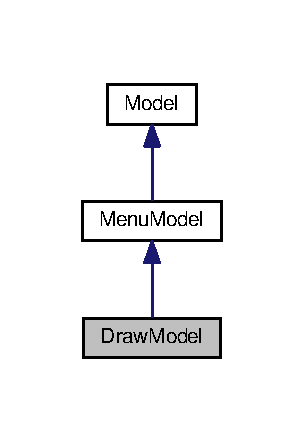
\includegraphics[width=146pt]{classDrawModel__inherit__graph}
\end{center}
\end{figure}


Collaboration diagram for Draw\-Model\-:
\nopagebreak
\begin{figure}[H]
\begin{center}
\leavevmode
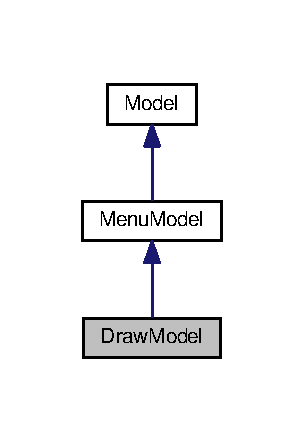
\includegraphics[width=146pt]{classDrawModel__coll__graph}
\end{center}
\end{figure}
\subsection*{Public Member Functions}
\begin{DoxyCompactItemize}
\item 
\hyperlink{classDrawModel_ad3a824bc973a552db96e0bce14ebc5de}{Draw\-Model} ()=default
\item 
\hyperlink{classDrawModel_aead59f7f6d9d39157176d730e0ab1f31}{$\sim$\-Draw\-Model} ()
\item 
void \hyperlink{classDrawModel_a29527786c01f93493af7cb38064d71c6}{draw\-Gliph} (\hyperlink{classGliph}{Gliph} $\ast$gliph\-Name)
\item 
void \hyperlink{classDrawModel_aaabab93258cb0abe8303b1f6a406b5d4}{delete\-Gliph} (\hyperlink{classGliph}{Gliph} $\ast$gliph\-Name)
\item 
virtual std\-::string \hyperlink{classDrawModel_a64d70716532d50216910f4c37b75da32}{print\-State} ()
\end{DoxyCompactItemize}
\subsection*{Additional Inherited Members}


\subsection{Constructor \& Destructor Documentation}
\hypertarget{classDrawModel_ad3a824bc973a552db96e0bce14ebc5de}{\index{Draw\-Model@{Draw\-Model}!Draw\-Model@{Draw\-Model}}
\index{Draw\-Model@{Draw\-Model}!DrawModel@{Draw\-Model}}
\subsubsection[{Draw\-Model}]{\setlength{\rightskip}{0pt plus 5cm}Draw\-Model\-::\-Draw\-Model (
\begin{DoxyParamCaption}
{}
\end{DoxyParamCaption}
)\hspace{0.3cm}{\ttfamily [default]}}}\label{classDrawModel_ad3a824bc973a552db96e0bce14ebc5de}
\hypertarget{classDrawModel_aead59f7f6d9d39157176d730e0ab1f31}{\index{Draw\-Model@{Draw\-Model}!$\sim$\-Draw\-Model@{$\sim$\-Draw\-Model}}
\index{$\sim$\-Draw\-Model@{$\sim$\-Draw\-Model}!DrawModel@{Draw\-Model}}
\subsubsection[{$\sim$\-Draw\-Model}]{\setlength{\rightskip}{0pt plus 5cm}Draw\-Model\-::$\sim$\-Draw\-Model (
\begin{DoxyParamCaption}
{}
\end{DoxyParamCaption}
)\hspace{0.3cm}{\ttfamily [inline]}}}\label{classDrawModel_aead59f7f6d9d39157176d730e0ab1f31}


\subsection{Member Function Documentation}
\hypertarget{classDrawModel_aaabab93258cb0abe8303b1f6a406b5d4}{\index{Draw\-Model@{Draw\-Model}!delete\-Gliph@{delete\-Gliph}}
\index{delete\-Gliph@{delete\-Gliph}!DrawModel@{Draw\-Model}}
\subsubsection[{delete\-Gliph}]{\setlength{\rightskip}{0pt plus 5cm}void Draw\-Model\-::delete\-Gliph (
\begin{DoxyParamCaption}
\item[{{\bf Gliph} $\ast$}]{gliph\-Name}
\end{DoxyParamCaption}
)}}\label{classDrawModel_aaabab93258cb0abe8303b1f6a406b5d4}
\hypertarget{classDrawModel_a29527786c01f93493af7cb38064d71c6}{\index{Draw\-Model@{Draw\-Model}!draw\-Gliph@{draw\-Gliph}}
\index{draw\-Gliph@{draw\-Gliph}!DrawModel@{Draw\-Model}}
\subsubsection[{draw\-Gliph}]{\setlength{\rightskip}{0pt plus 5cm}void Draw\-Model\-::draw\-Gliph (
\begin{DoxyParamCaption}
\item[{{\bf Gliph} $\ast$}]{gliph\-Name}
\end{DoxyParamCaption}
)}}\label{classDrawModel_a29527786c01f93493af7cb38064d71c6}
\hypertarget{classDrawModel_a64d70716532d50216910f4c37b75da32}{\index{Draw\-Model@{Draw\-Model}!print\-State@{print\-State}}
\index{print\-State@{print\-State}!DrawModel@{Draw\-Model}}
\subsubsection[{print\-State}]{\setlength{\rightskip}{0pt plus 5cm}std\-::string Draw\-Model\-::print\-State (
\begin{DoxyParamCaption}
{}
\end{DoxyParamCaption}
)\hspace{0.3cm}{\ttfamily [virtual]}}}\label{classDrawModel_a64d70716532d50216910f4c37b75da32}


Reimplemented from \hyperlink{classMenuModel_ab49130e41f188e5c632c4681961d9415}{Menu\-Model}.



The documentation for this class was generated from the following files\-:\begin{DoxyCompactItemize}
\item 
/home/travis/build/senyacherenkov/lesson\-\_\-12\-\_\-homework/\hyperlink{model_8h}{model.\-h}\item 
/home/travis/build/senyacherenkov/lesson\-\_\-12\-\_\-homework/\hyperlink{model_8cpp}{model.\-cpp}\end{DoxyCompactItemize}

\hypertarget{classGlyph}{\section{Glyph Class Reference}
\label{classGlyph}\index{Glyph@{Glyph}}
}


{\ttfamily \#include $<$gliph.\-h$>$}



Inheritance diagram for Glyph\-:
\nopagebreak
\begin{figure}[H]
\begin{center}
\leavevmode
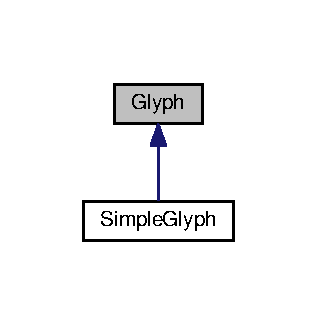
\includegraphics[width=152pt]{classGlyph__inherit__graph}
\end{center}
\end{figure}
\subsection*{Public Member Functions}
\begin{DoxyCompactItemize}
\item 
\hyperlink{classGlyph_ad9bd394041828e7ea6599e4cc0f9f09e}{Glyph} (std\-::string description)
\item 
std\-::string \hyperlink{classGlyph_a486c653c91f1b1a194544f6280d0b654}{get\-Description} ()
\end{DoxyCompactItemize}


\subsection{Constructor \& Destructor Documentation}
\hypertarget{classGlyph_ad9bd394041828e7ea6599e4cc0f9f09e}{\index{Glyph@{Glyph}!Glyph@{Glyph}}
\index{Glyph@{Glyph}!Glyph@{Glyph}}
\subsubsection[{Glyph}]{\setlength{\rightskip}{0pt plus 5cm}Glyph\-::\-Glyph (
\begin{DoxyParamCaption}
\item[{std\-::string}]{description}
\end{DoxyParamCaption}
)\hspace{0.3cm}{\ttfamily [inline]}}}\label{classGlyph_ad9bd394041828e7ea6599e4cc0f9f09e}


\subsection{Member Function Documentation}
\hypertarget{classGlyph_a486c653c91f1b1a194544f6280d0b654}{\index{Glyph@{Glyph}!get\-Description@{get\-Description}}
\index{get\-Description@{get\-Description}!Glyph@{Glyph}}
\subsubsection[{get\-Description}]{\setlength{\rightskip}{0pt plus 5cm}std\-::string Glyph\-::get\-Description (
\begin{DoxyParamCaption}
{}
\end{DoxyParamCaption}
)\hspace{0.3cm}{\ttfamily [inline]}}}\label{classGlyph_a486c653c91f1b1a194544f6280d0b654}


The documentation for this class was generated from the following file\-:\begin{DoxyCompactItemize}
\item 
/home/travis/build/senyacherenkov/lesson\-\_\-12\-\_\-homework/\hyperlink{gliph_8h}{gliph.\-h}\end{DoxyCompactItemize}

\hypertarget{classMenuController}{\section{Menu\-Controller Class Reference}
\label{classMenuController}\index{Menu\-Controller@{Menu\-Controller}}
}


{\ttfamily \#include $<$controller.\-h$>$}

\subsection*{Public Member Functions}
\begin{DoxyCompactItemize}
\item 
\hyperlink{classMenuController_a51fa85e8ac5858efc9129002d8104544}{Menu\-Controller} (\hyperlink{classMenuModel}{Menu\-Model} \&model)
\item 
void \hyperlink{classMenuController_a363b3b1f1ec549bad12d9c21e735199e}{create\-New\-Document} (std\-::string doc\-Name)
\item 
void \hyperlink{classMenuController_a4f1afff77b046474eb1d2248a7c1e53e}{import\-Document} (std\-::string doc\-Name)
\item 
std\-::string \hyperlink{classMenuController_ae117eda1c1bc63bc75cd5475d570e561}{export\-Document} ()
\end{DoxyCompactItemize}


\subsection{Constructor \& Destructor Documentation}
\hypertarget{classMenuController_a51fa85e8ac5858efc9129002d8104544}{\index{Menu\-Controller@{Menu\-Controller}!Menu\-Controller@{Menu\-Controller}}
\index{Menu\-Controller@{Menu\-Controller}!MenuController@{Menu\-Controller}}
\subsubsection[{Menu\-Controller}]{\setlength{\rightskip}{0pt plus 5cm}Menu\-Controller\-::\-Menu\-Controller (
\begin{DoxyParamCaption}
\item[{{\bf Menu\-Model} \&}]{model}
\end{DoxyParamCaption}
)\hspace{0.3cm}{\ttfamily [inline]}}}\label{classMenuController_a51fa85e8ac5858efc9129002d8104544}


\subsection{Member Function Documentation}
\hypertarget{classMenuController_a363b3b1f1ec549bad12d9c21e735199e}{\index{Menu\-Controller@{Menu\-Controller}!create\-New\-Document@{create\-New\-Document}}
\index{create\-New\-Document@{create\-New\-Document}!MenuController@{Menu\-Controller}}
\subsubsection[{create\-New\-Document}]{\setlength{\rightskip}{0pt plus 5cm}void Menu\-Controller\-::create\-New\-Document (
\begin{DoxyParamCaption}
\item[{std\-::string}]{doc\-Name}
\end{DoxyParamCaption}
)\hspace{0.3cm}{\ttfamily [inline]}}}\label{classMenuController_a363b3b1f1ec549bad12d9c21e735199e}
\hypertarget{classMenuController_ae117eda1c1bc63bc75cd5475d570e561}{\index{Menu\-Controller@{Menu\-Controller}!export\-Document@{export\-Document}}
\index{export\-Document@{export\-Document}!MenuController@{Menu\-Controller}}
\subsubsection[{export\-Document}]{\setlength{\rightskip}{0pt plus 5cm}std\-::string Menu\-Controller\-::export\-Document (
\begin{DoxyParamCaption}
{}
\end{DoxyParamCaption}
)\hspace{0.3cm}{\ttfamily [inline]}}}\label{classMenuController_ae117eda1c1bc63bc75cd5475d570e561}
\hypertarget{classMenuController_a4f1afff77b046474eb1d2248a7c1e53e}{\index{Menu\-Controller@{Menu\-Controller}!import\-Document@{import\-Document}}
\index{import\-Document@{import\-Document}!MenuController@{Menu\-Controller}}
\subsubsection[{import\-Document}]{\setlength{\rightskip}{0pt plus 5cm}void Menu\-Controller\-::import\-Document (
\begin{DoxyParamCaption}
\item[{std\-::string}]{doc\-Name}
\end{DoxyParamCaption}
)\hspace{0.3cm}{\ttfamily [inline]}}}\label{classMenuController_a4f1afff77b046474eb1d2248a7c1e53e}


The documentation for this class was generated from the following file\-:\begin{DoxyCompactItemize}
\item 
/home/travis/build/senyacherenkov/lesson\-\_\-12\-\_\-homework/\hyperlink{controller_8h}{controller.\-h}\end{DoxyCompactItemize}

\hypertarget{classMenuModel}{\section{Menu\-Model Class Reference}
\label{classMenuModel}\index{Menu\-Model@{Menu\-Model}}
}


{\ttfamily \#include $<$model.\-h$>$}



Inheritance diagram for Menu\-Model\-:
\nopagebreak
\begin{figure}[H]
\begin{center}
\leavevmode
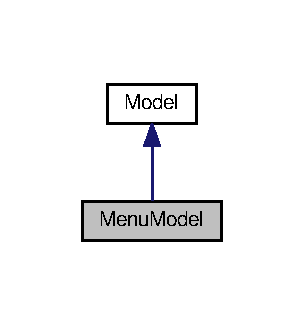
\includegraphics[width=146pt]{classMenuModel__inherit__graph}
\end{center}
\end{figure}


Collaboration diagram for Menu\-Model\-:
\nopagebreak
\begin{figure}[H]
\begin{center}
\leavevmode
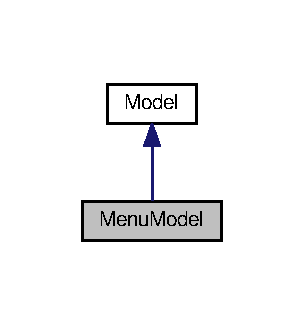
\includegraphics[width=146pt]{classMenuModel__coll__graph}
\end{center}
\end{figure}
\subsection*{Public Member Functions}
\begin{DoxyCompactItemize}
\item 
\hyperlink{classMenuModel_aed6e639866f25ae4ab388302cf51ac77}{Menu\-Model} ()=default
\item 
\hyperlink{classMenuModel_a302ddb32e707719e85d559979f0b5d97}{$\sim$\-Menu\-Model} ()
\item 
void \hyperlink{classMenuModel_ad9b8d1e30f024c6a2283d1c91822bdd2}{create\-Document} (std\-::string \&doc\-Name)
\item 
void \hyperlink{classMenuModel_a95f08e56638248ef87aecd4d562ba44b}{import\-Document} (std\-::string \&doc\-Name)
\item 
void \hyperlink{classMenuModel_a3533d1ef3d28bb399e9e276b9aa81007}{export\-Document} (std\-::string \&doc\-Name)
\item 
\hyperlink{classGlyph}{Glyph} $\ast$ \hyperlink{classMenuModel_a73a5b58296b95f8ee55fc6581f5a3002}{create\-Glyph} (\hyperlink{gliph_8h_a84dea1dd1afdc2f1990fe2b14d971b6e}{Glyph\-Type} glyph, std\-::string description)
\item 
virtual std\-::string \hyperlink{classMenuModel_ab49130e41f188e5c632c4681961d9415}{print\-State} ()
\end{DoxyCompactItemize}
\subsection*{Additional Inherited Members}


\subsection{Constructor \& Destructor Documentation}
\hypertarget{classMenuModel_aed6e639866f25ae4ab388302cf51ac77}{\index{Menu\-Model@{Menu\-Model}!Menu\-Model@{Menu\-Model}}
\index{Menu\-Model@{Menu\-Model}!MenuModel@{Menu\-Model}}
\subsubsection[{Menu\-Model}]{\setlength{\rightskip}{0pt plus 5cm}Menu\-Model\-::\-Menu\-Model (
\begin{DoxyParamCaption}
{}
\end{DoxyParamCaption}
)\hspace{0.3cm}{\ttfamily [default]}}}\label{classMenuModel_aed6e639866f25ae4ab388302cf51ac77}
\hypertarget{classMenuModel_a302ddb32e707719e85d559979f0b5d97}{\index{Menu\-Model@{Menu\-Model}!$\sim$\-Menu\-Model@{$\sim$\-Menu\-Model}}
\index{$\sim$\-Menu\-Model@{$\sim$\-Menu\-Model}!MenuModel@{Menu\-Model}}
\subsubsection[{$\sim$\-Menu\-Model}]{\setlength{\rightskip}{0pt plus 5cm}Menu\-Model\-::$\sim$\-Menu\-Model (
\begin{DoxyParamCaption}
{}
\end{DoxyParamCaption}
)\hspace{0.3cm}{\ttfamily [inline]}}}\label{classMenuModel_a302ddb32e707719e85d559979f0b5d97}


\subsection{Member Function Documentation}
\hypertarget{classMenuModel_ad9b8d1e30f024c6a2283d1c91822bdd2}{\index{Menu\-Model@{Menu\-Model}!create\-Document@{create\-Document}}
\index{create\-Document@{create\-Document}!MenuModel@{Menu\-Model}}
\subsubsection[{create\-Document}]{\setlength{\rightskip}{0pt plus 5cm}void Menu\-Model\-::create\-Document (
\begin{DoxyParamCaption}
\item[{std\-::string \&}]{doc\-Name}
\end{DoxyParamCaption}
)}}\label{classMenuModel_ad9b8d1e30f024c6a2283d1c91822bdd2}
\hypertarget{classMenuModel_a73a5b58296b95f8ee55fc6581f5a3002}{\index{Menu\-Model@{Menu\-Model}!create\-Glyph@{create\-Glyph}}
\index{create\-Glyph@{create\-Glyph}!MenuModel@{Menu\-Model}}
\subsubsection[{create\-Glyph}]{\setlength{\rightskip}{0pt plus 5cm}{\bf Glyph} $\ast$ Menu\-Model\-::create\-Glyph (
\begin{DoxyParamCaption}
\item[{{\bf Glyph\-Type}}]{glyph, }
\item[{std\-::string}]{description}
\end{DoxyParamCaption}
)}}\label{classMenuModel_a73a5b58296b95f8ee55fc6581f5a3002}
\hypertarget{classMenuModel_a3533d1ef3d28bb399e9e276b9aa81007}{\index{Menu\-Model@{Menu\-Model}!export\-Document@{export\-Document}}
\index{export\-Document@{export\-Document}!MenuModel@{Menu\-Model}}
\subsubsection[{export\-Document}]{\setlength{\rightskip}{0pt plus 5cm}void Menu\-Model\-::export\-Document (
\begin{DoxyParamCaption}
\item[{std\-::string \&}]{doc\-Name}
\end{DoxyParamCaption}
)}}\label{classMenuModel_a3533d1ef3d28bb399e9e276b9aa81007}
\hypertarget{classMenuModel_a95f08e56638248ef87aecd4d562ba44b}{\index{Menu\-Model@{Menu\-Model}!import\-Document@{import\-Document}}
\index{import\-Document@{import\-Document}!MenuModel@{Menu\-Model}}
\subsubsection[{import\-Document}]{\setlength{\rightskip}{0pt plus 5cm}void Menu\-Model\-::import\-Document (
\begin{DoxyParamCaption}
\item[{std\-::string \&}]{doc\-Name}
\end{DoxyParamCaption}
)}}\label{classMenuModel_a95f08e56638248ef87aecd4d562ba44b}
\hypertarget{classMenuModel_ab49130e41f188e5c632c4681961d9415}{\index{Menu\-Model@{Menu\-Model}!print\-State@{print\-State}}
\index{print\-State@{print\-State}!MenuModel@{Menu\-Model}}
\subsubsection[{print\-State}]{\setlength{\rightskip}{0pt plus 5cm}std\-::string Menu\-Model\-::print\-State (
\begin{DoxyParamCaption}
{}
\end{DoxyParamCaption}
)\hspace{0.3cm}{\ttfamily [virtual]}}}\label{classMenuModel_ab49130e41f188e5c632c4681961d9415}


Implements \hyperlink{classModel_a853995c3960bc17b4df783d76ca5dfeb}{Model}.



The documentation for this class was generated from the following files\-:\begin{DoxyCompactItemize}
\item 
/home/travis/build/senyacherenkov/lesson\-\_\-12\-\_\-homework/\hyperlink{model_8h}{model.\-h}\item 
/home/travis/build/senyacherenkov/lesson\-\_\-12\-\_\-homework/\hyperlink{model_8cpp}{model.\-cpp}\end{DoxyCompactItemize}

\hypertarget{classModel}{\section{Model Class Reference}
\label{classModel}\index{Model@{Model}}
}


{\ttfamily \#include $<$model.\-h$>$}



Inheritance diagram for Model\-:
\nopagebreak
\begin{figure}[H]
\begin{center}
\leavevmode
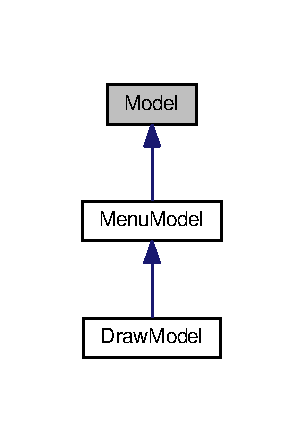
\includegraphics[width=146pt]{classModel__inherit__graph}
\end{center}
\end{figure}
\subsection*{Public Member Functions}
\begin{DoxyCompactItemize}
\item 
virtual \hyperlink{classModel_ad6ebd2062a0b823db841a0b88baac4c0}{$\sim$\-Model} ()
\item 
void \hyperlink{classModel_af12598805e6271d9c64f90d31c15f7d3}{connect} (\hyperlink{model_8h_aac0c1ba55260a4d57385cf6a95c5df0a}{Listener} view)
\item 
virtual std\-::string \hyperlink{classModel_a853995c3960bc17b4df783d76ca5dfeb}{print\-State} ()=0
\end{DoxyCompactItemize}
\subsection*{Protected Member Functions}
\begin{DoxyCompactItemize}
\item 
void \hyperlink{classModel_a9f6a71b1dbc4fb979781f355ae9c78d2}{notify} ()
\end{DoxyCompactItemize}
\subsection*{Protected Attributes}
\begin{DoxyCompactItemize}
\item 
std\-::string \hyperlink{classModel_a4f8aa4311a54d069a54dc2626461163f}{m\-\_\-doc\-Name}
\end{DoxyCompactItemize}


\subsection{Constructor \& Destructor Documentation}
\hypertarget{classModel_ad6ebd2062a0b823db841a0b88baac4c0}{\index{Model@{Model}!$\sim$\-Model@{$\sim$\-Model}}
\index{$\sim$\-Model@{$\sim$\-Model}!Model@{Model}}
\subsubsection[{$\sim$\-Model}]{\setlength{\rightskip}{0pt plus 5cm}Model\-::$\sim$\-Model (
\begin{DoxyParamCaption}
{}
\end{DoxyParamCaption}
)\hspace{0.3cm}{\ttfamily [virtual]}}}\label{classModel_ad6ebd2062a0b823db841a0b88baac4c0}


\subsection{Member Function Documentation}
\hypertarget{classModel_af12598805e6271d9c64f90d31c15f7d3}{\index{Model@{Model}!connect@{connect}}
\index{connect@{connect}!Model@{Model}}
\subsubsection[{connect}]{\setlength{\rightskip}{0pt plus 5cm}void Model\-::connect (
\begin{DoxyParamCaption}
\item[{{\bf Listener}}]{view}
\end{DoxyParamCaption}
)\hspace{0.3cm}{\ttfamily [inline]}}}\label{classModel_af12598805e6271d9c64f90d31c15f7d3}
\hypertarget{classModel_a9f6a71b1dbc4fb979781f355ae9c78d2}{\index{Model@{Model}!notify@{notify}}
\index{notify@{notify}!Model@{Model}}
\subsubsection[{notify}]{\setlength{\rightskip}{0pt plus 5cm}void Model\-::notify (
\begin{DoxyParamCaption}
{}
\end{DoxyParamCaption}
)\hspace{0.3cm}{\ttfamily [protected]}}}\label{classModel_a9f6a71b1dbc4fb979781f355ae9c78d2}
\hypertarget{classModel_a853995c3960bc17b4df783d76ca5dfeb}{\index{Model@{Model}!print\-State@{print\-State}}
\index{print\-State@{print\-State}!Model@{Model}}
\subsubsection[{print\-State}]{\setlength{\rightskip}{0pt plus 5cm}virtual std\-::string Model\-::print\-State (
\begin{DoxyParamCaption}
{}
\end{DoxyParamCaption}
)\hspace{0.3cm}{\ttfamily [pure virtual]}}}\label{classModel_a853995c3960bc17b4df783d76ca5dfeb}


Implemented in \hyperlink{classDrawModel_a64d70716532d50216910f4c37b75da32}{Draw\-Model}, and \hyperlink{classMenuModel_ab49130e41f188e5c632c4681961d9415}{Menu\-Model}.



\subsection{Member Data Documentation}
\hypertarget{classModel_a4f8aa4311a54d069a54dc2626461163f}{\index{Model@{Model}!m\-\_\-doc\-Name@{m\-\_\-doc\-Name}}
\index{m\-\_\-doc\-Name@{m\-\_\-doc\-Name}!Model@{Model}}
\subsubsection[{m\-\_\-doc\-Name}]{\setlength{\rightskip}{0pt plus 5cm}std\-::string Model\-::m\-\_\-doc\-Name\hspace{0.3cm}{\ttfamily [protected]}}}\label{classModel_a4f8aa4311a54d069a54dc2626461163f}


The documentation for this class was generated from the following files\-:\begin{DoxyCompactItemize}
\item 
/home/travis/build/senyacherenkov/lesson\-\_\-12\-\_\-homework/\hyperlink{model_8h}{model.\-h}\item 
/home/travis/build/senyacherenkov/lesson\-\_\-12\-\_\-homework/\hyperlink{model_8cpp}{model.\-cpp}\end{DoxyCompactItemize}

\hypertarget{classSimpleGlyph}{\section{Simple\-Glyph Class Reference}
\label{classSimpleGlyph}\index{Simple\-Glyph@{Simple\-Glyph}}
}


{\ttfamily \#include $<$gliph.\-h$>$}



Inheritance diagram for Simple\-Glyph\-:
\nopagebreak
\begin{figure}[H]
\begin{center}
\leavevmode
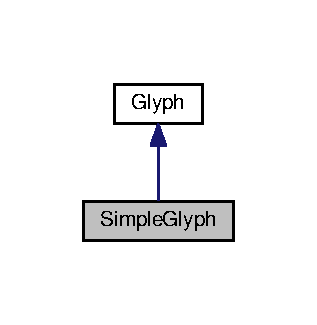
\includegraphics[width=152pt]{classSimpleGlyph__inherit__graph}
\end{center}
\end{figure}


Collaboration diagram for Simple\-Glyph\-:
\nopagebreak
\begin{figure}[H]
\begin{center}
\leavevmode
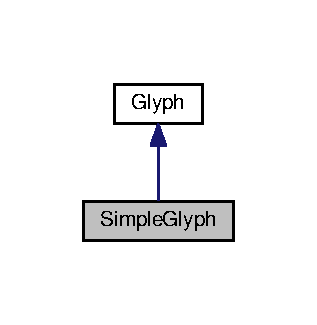
\includegraphics[width=152pt]{classSimpleGlyph__coll__graph}
\end{center}
\end{figure}
\subsection*{Public Member Functions}
\begin{DoxyCompactItemize}
\item 
\hyperlink{classSimpleGlyph_af74a93771a158ebf07a85b73d5c899da}{Simple\-Glyph} (std\-::string description)
\end{DoxyCompactItemize}


\subsection{Constructor \& Destructor Documentation}
\hypertarget{classSimpleGlyph_af74a93771a158ebf07a85b73d5c899da}{\index{Simple\-Glyph@{Simple\-Glyph}!Simple\-Glyph@{Simple\-Glyph}}
\index{Simple\-Glyph@{Simple\-Glyph}!SimpleGlyph@{Simple\-Glyph}}
\subsubsection[{Simple\-Glyph}]{\setlength{\rightskip}{0pt plus 5cm}Simple\-Glyph\-::\-Simple\-Glyph (
\begin{DoxyParamCaption}
\item[{std\-::string}]{description}
\end{DoxyParamCaption}
)\hspace{0.3cm}{\ttfamily [inline]}}}\label{classSimpleGlyph_af74a93771a158ebf07a85b73d5c899da}


The documentation for this class was generated from the following file\-:\begin{DoxyCompactItemize}
\item 
/home/travis/build/senyacherenkov/lesson\-\_\-12\-\_\-homework/\hyperlink{gliph_8h}{gliph.\-h}\end{DoxyCompactItemize}

\hypertarget{classView}{\section{View Class Reference}
\label{classView}\index{View@{View}}
}


{\ttfamily \#include $<$view.\-h$>$}

\subsection*{Public Member Functions}
\begin{DoxyCompactItemize}
\item 
\hyperlink{classView_a9661c7b63a0988067c48fe7e56171bcd}{View} ()=default
\item 
void \hyperlink{classView_adbc2c6a372ebdd3bd8d75dd158b9ad89}{print\-State\-Of\-Document} (\hyperlink{classModel}{Model} $\ast$model)
\end{DoxyCompactItemize}


\subsection{Constructor \& Destructor Documentation}
\hypertarget{classView_a9661c7b63a0988067c48fe7e56171bcd}{\index{View@{View}!View@{View}}
\index{View@{View}!View@{View}}
\subsubsection[{View}]{\setlength{\rightskip}{0pt plus 5cm}View\-::\-View (
\begin{DoxyParamCaption}
{}
\end{DoxyParamCaption}
)\hspace{0.3cm}{\ttfamily [default]}}}\label{classView_a9661c7b63a0988067c48fe7e56171bcd}


\subsection{Member Function Documentation}
\hypertarget{classView_adbc2c6a372ebdd3bd8d75dd158b9ad89}{\index{View@{View}!print\-State\-Of\-Document@{print\-State\-Of\-Document}}
\index{print\-State\-Of\-Document@{print\-State\-Of\-Document}!View@{View}}
\subsubsection[{print\-State\-Of\-Document}]{\setlength{\rightskip}{0pt plus 5cm}void View\-::print\-State\-Of\-Document (
\begin{DoxyParamCaption}
\item[{{\bf Model} $\ast$}]{model}
\end{DoxyParamCaption}
)\hspace{0.3cm}{\ttfamily [inline]}}}\label{classView_adbc2c6a372ebdd3bd8d75dd158b9ad89}


The documentation for this class was generated from the following file\-:\begin{DoxyCompactItemize}
\item 
/home/travis/build/senyacherenkov/lesson\-\_\-12\-\_\-homework/\hyperlink{view_8h}{view.\-h}\end{DoxyCompactItemize}

\chapter{File Documentation}
\hypertarget{controller_8h}{\section{/home/travis/build/senyacherenkov/lesson\-\_\-12\-\_\-homework/controller.h File Reference}
\label{controller_8h}\index{/home/travis/build/senyacherenkov/lesson\-\_\-12\-\_\-homework/controller.\-h@{/home/travis/build/senyacherenkov/lesson\-\_\-12\-\_\-homework/controller.\-h}}
}
{\ttfamily \#include \char`\"{}model.\-h\char`\"{}}\\*
{\ttfamily \#include \char`\"{}gliph.\-h\char`\"{}}\\*
Include dependency graph for controller.\-h\-:
\nopagebreak
\begin{figure}[H]
\begin{center}
\leavevmode
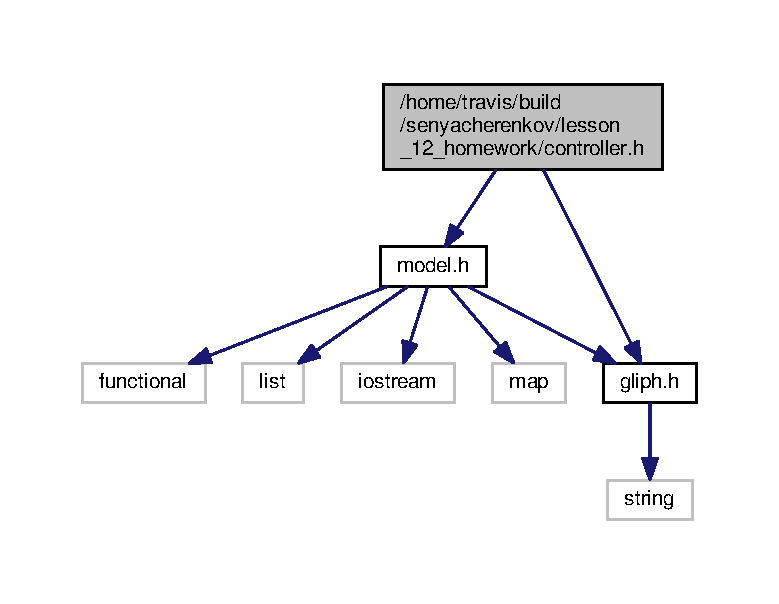
\includegraphics[width=350pt]{controller_8h__incl}
\end{center}
\end{figure}
This graph shows which files directly or indirectly include this file\-:
\nopagebreak
\begin{figure}[H]
\begin{center}
\leavevmode
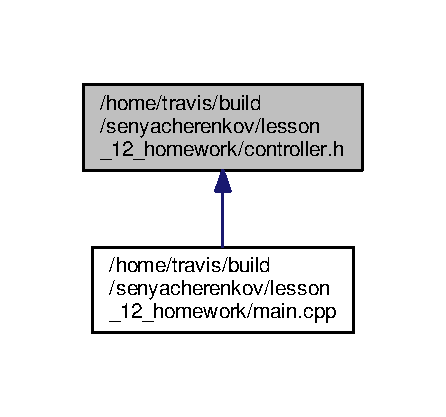
\includegraphics[width=214pt]{controller_8h__dep__incl}
\end{center}
\end{figure}
\subsection*{Classes}
\begin{DoxyCompactItemize}
\item 
class \hyperlink{classMenuController}{Menu\-Controller}
\item 
class \hyperlink{classDrawController}{Draw\-Controller}
\end{DoxyCompactItemize}

\hypertarget{gliph_8h}{\section{/home/travis/build/senyacherenkov/lesson\-\_\-12\-\_\-homework/gliph.h File Reference}
\label{gliph_8h}\index{/home/travis/build/senyacherenkov/lesson\-\_\-12\-\_\-homework/gliph.\-h@{/home/travis/build/senyacherenkov/lesson\-\_\-12\-\_\-homework/gliph.\-h}}
}
{\ttfamily \#include $<$string$>$}\\*
Include dependency graph for gliph.\-h\-:
\nopagebreak
\begin{figure}[H]
\begin{center}
\leavevmode
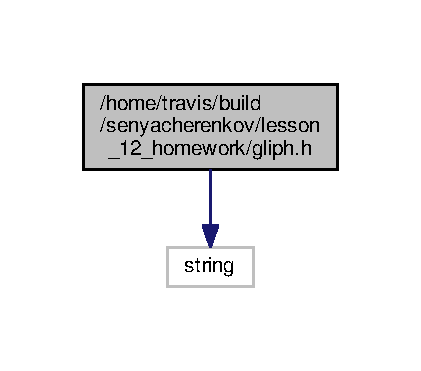
\includegraphics[width=202pt]{gliph_8h__incl}
\end{center}
\end{figure}
This graph shows which files directly or indirectly include this file\-:
\nopagebreak
\begin{figure}[H]
\begin{center}
\leavevmode
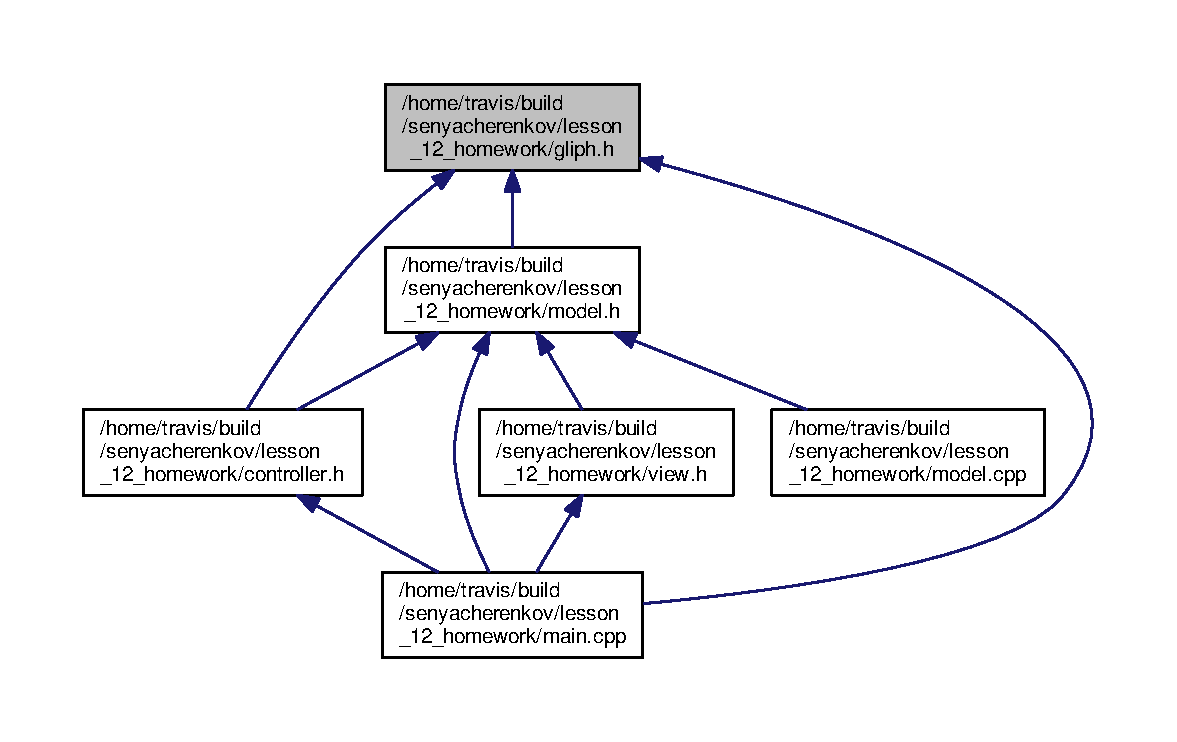
\includegraphics[width=350pt]{gliph_8h__dep__incl}
\end{center}
\end{figure}
\subsection*{Classes}
\begin{DoxyCompactItemize}
\item 
class \hyperlink{classGlyph}{Glyph}
\item 
class \hyperlink{classSimpleGlyph}{Simple\-Glyph}
\end{DoxyCompactItemize}
\subsection*{Enumerations}
\begin{DoxyCompactItemize}
\item 
enum \hyperlink{gliph_8h_a84dea1dd1afdc2f1990fe2b14d971b6e}{Glyph\-Type} \{ \hyperlink{gliph_8h_a84dea1dd1afdc2f1990fe2b14d971b6ea9ae76c089db1975bb55eaf939896ad16}{Glyph\-Type\-::\-S\-I\-M\-P\-L\-E\-\_\-\-G\-L\-Y\-P\-H}, 
\hyperlink{gliph_8h_a84dea1dd1afdc2f1990fe2b14d971b6ea7a2b1b3f2e0547d56de9996cd42130f4}{Glyph\-Type\-::\-O\-T\-H\-E\-R\-\_\-\-G\-L\-Y\-P\-H}
 \}
\end{DoxyCompactItemize}


\subsection{Enumeration Type Documentation}
\hypertarget{gliph_8h_a84dea1dd1afdc2f1990fe2b14d971b6e}{\index{gliph.\-h@{gliph.\-h}!Glyph\-Type@{Glyph\-Type}}
\index{Glyph\-Type@{Glyph\-Type}!gliph.h@{gliph.\-h}}
\subsubsection[{Glyph\-Type}]{\setlength{\rightskip}{0pt plus 5cm}enum {\bf Glyph\-Type}\hspace{0.3cm}{\ttfamily [strong]}}}\label{gliph_8h_a84dea1dd1afdc2f1990fe2b14d971b6e}
\begin{Desc}
\item[Enumerator]\par
\begin{description}
\index{S\-I\-M\-P\-L\-E\-\_\-\-G\-L\-Y\-P\-H@{S\-I\-M\-P\-L\-E\-\_\-\-G\-L\-Y\-P\-H}!gliph.\-h@{gliph.\-h}}\index{gliph.\-h@{gliph.\-h}!S\-I\-M\-P\-L\-E\-\_\-\-G\-L\-Y\-P\-H@{S\-I\-M\-P\-L\-E\-\_\-\-G\-L\-Y\-P\-H}}\item[{\em 
\hypertarget{gliph_8h_a84dea1dd1afdc2f1990fe2b14d971b6ea9ae76c089db1975bb55eaf939896ad16}{S\-I\-M\-P\-L\-E\-\_\-\-G\-L\-Y\-P\-H}\label{gliph_8h_a84dea1dd1afdc2f1990fe2b14d971b6ea9ae76c089db1975bb55eaf939896ad16}
}]\index{O\-T\-H\-E\-R\-\_\-\-G\-L\-Y\-P\-H@{O\-T\-H\-E\-R\-\_\-\-G\-L\-Y\-P\-H}!gliph.\-h@{gliph.\-h}}\index{gliph.\-h@{gliph.\-h}!O\-T\-H\-E\-R\-\_\-\-G\-L\-Y\-P\-H@{O\-T\-H\-E\-R\-\_\-\-G\-L\-Y\-P\-H}}\item[{\em 
\hypertarget{gliph_8h_a84dea1dd1afdc2f1990fe2b14d971b6ea7a2b1b3f2e0547d56de9996cd42130f4}{O\-T\-H\-E\-R\-\_\-\-G\-L\-Y\-P\-H}\label{gliph_8h_a84dea1dd1afdc2f1990fe2b14d971b6ea7a2b1b3f2e0547d56de9996cd42130f4}
}]\end{description}
\end{Desc}

\hypertarget{main_8cpp}{\section{/home/travis/build/senyacherenkov/lesson\-\_\-12\-\_\-homework/main.cpp File Reference}
\label{main_8cpp}\index{/home/travis/build/senyacherenkov/lesson\-\_\-12\-\_\-homework/main.\-cpp@{/home/travis/build/senyacherenkov/lesson\-\_\-12\-\_\-homework/main.\-cpp}}
}
{\ttfamily \#include $<$iostream$>$}\\*
{\ttfamily \#include \char`\"{}controller.\-h\char`\"{}}\\*
{\ttfamily \#include \char`\"{}model.\-h\char`\"{}}\\*
{\ttfamily \#include \char`\"{}view.\-h\char`\"{}}\\*
{\ttfamily \#include \char`\"{}gliph.\-h\char`\"{}}\\*
Include dependency graph for main.\-cpp\-:
\nopagebreak
\begin{figure}[H]
\begin{center}
\leavevmode
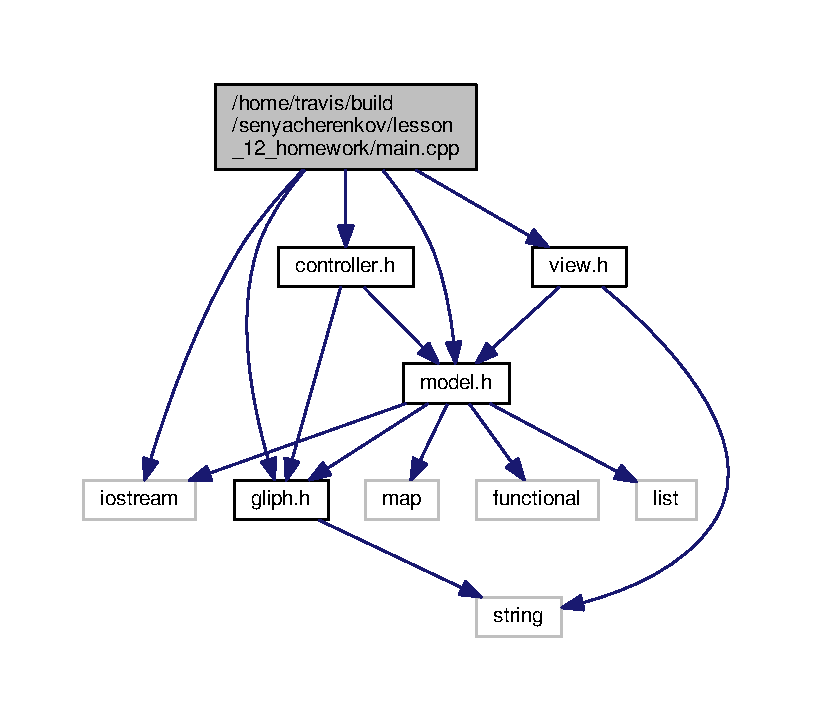
\includegraphics[width=350pt]{main_8cpp__incl}
\end{center}
\end{figure}
\subsection*{Functions}
\begin{DoxyCompactItemize}
\item 
int \hyperlink{main_8cpp_ae66f6b31b5ad750f1fe042a706a4e3d4}{main} ()
\end{DoxyCompactItemize}


\subsection{Function Documentation}
\hypertarget{main_8cpp_ae66f6b31b5ad750f1fe042a706a4e3d4}{\index{main.\-cpp@{main.\-cpp}!main@{main}}
\index{main@{main}!main.cpp@{main.\-cpp}}
\subsubsection[{main}]{\setlength{\rightskip}{0pt plus 5cm}int main (
\begin{DoxyParamCaption}
{}
\end{DoxyParamCaption}
)}}\label{main_8cpp_ae66f6b31b5ad750f1fe042a706a4e3d4}

\hypertarget{model_8cpp}{\section{/home/travis/build/senyacherenkov/lesson\-\_\-12\-\_\-homework/model.cpp File Reference}
\label{model_8cpp}\index{/home/travis/build/senyacherenkov/lesson\-\_\-12\-\_\-homework/model.\-cpp@{/home/travis/build/senyacherenkov/lesson\-\_\-12\-\_\-homework/model.\-cpp}}
}
{\ttfamily \#include \char`\"{}model.\-h\char`\"{}}\\*
Include dependency graph for model.\-cpp\-:
\nopagebreak
\begin{figure}[H]
\begin{center}
\leavevmode
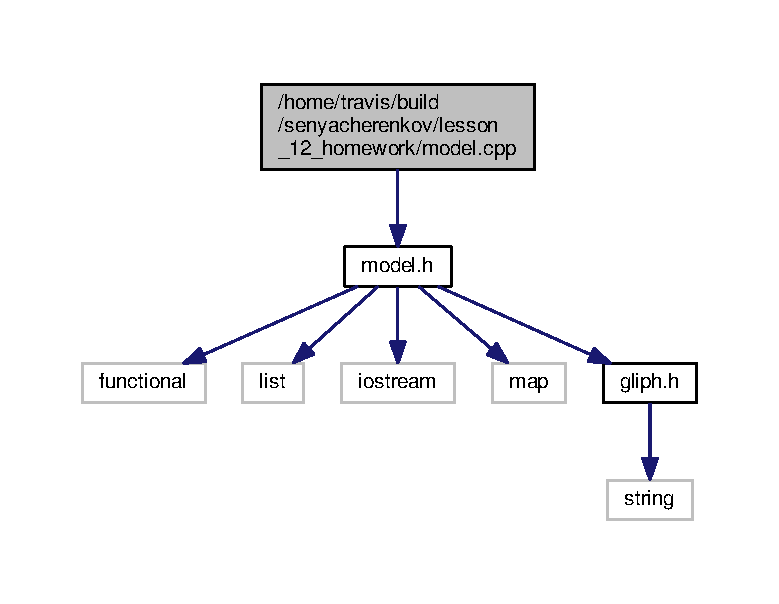
\includegraphics[width=350pt]{model_8cpp__incl}
\end{center}
\end{figure}

\hypertarget{model_8h}{\section{/home/travis/build/senyacherenkov/lesson\-\_\-12\-\_\-homework/model.h File Reference}
\label{model_8h}\index{/home/travis/build/senyacherenkov/lesson\-\_\-12\-\_\-homework/model.\-h@{/home/travis/build/senyacherenkov/lesson\-\_\-12\-\_\-homework/model.\-h}}
}
{\ttfamily \#include $<$functional$>$}\\*
{\ttfamily \#include $<$list$>$}\\*
{\ttfamily \#include $<$iostream$>$}\\*
{\ttfamily \#include $<$map$>$}\\*
{\ttfamily \#include \char`\"{}gliph.\-h\char`\"{}}\\*
Include dependency graph for model.\-h\-:
\nopagebreak
\begin{figure}[H]
\begin{center}
\leavevmode
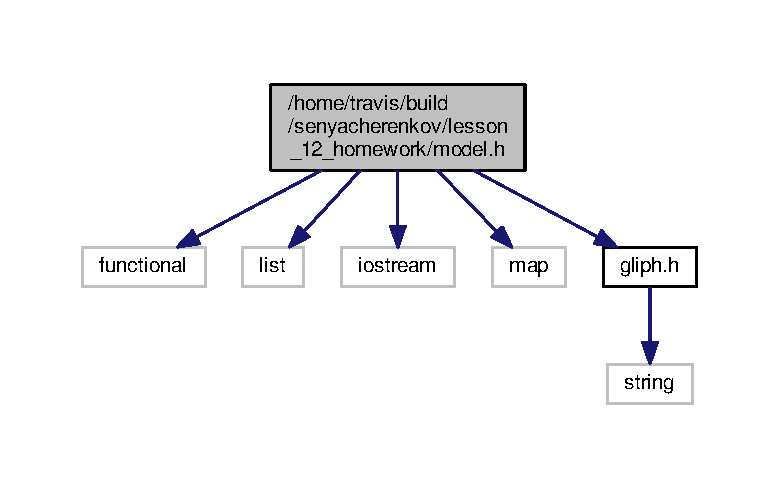
\includegraphics[width=350pt]{model_8h__incl}
\end{center}
\end{figure}
This graph shows which files directly or indirectly include this file\-:
\nopagebreak
\begin{figure}[H]
\begin{center}
\leavevmode
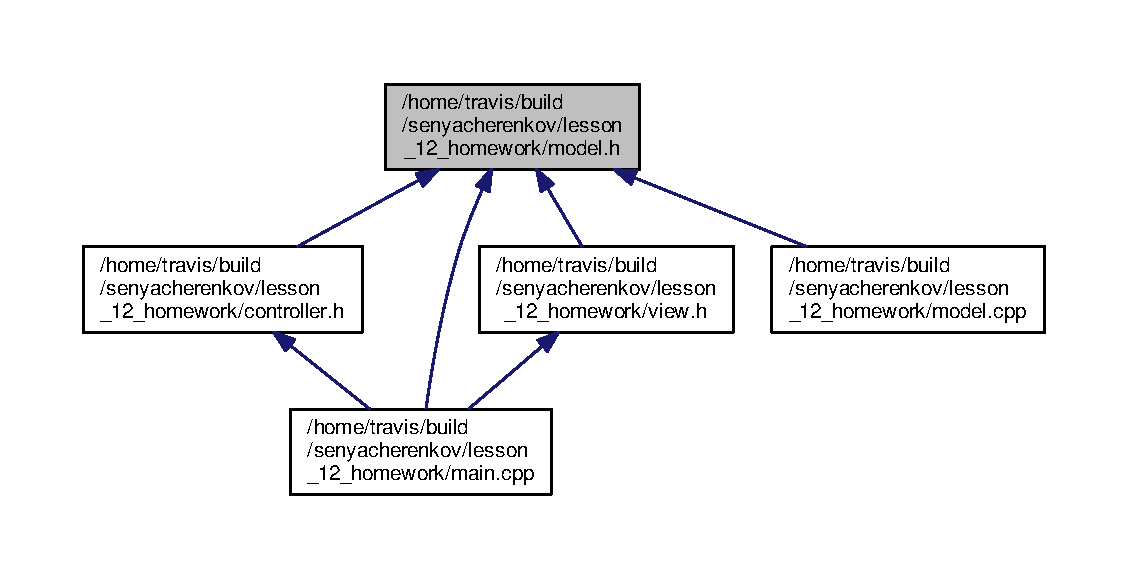
\includegraphics[width=350pt]{model_8h__dep__incl}
\end{center}
\end{figure}
\subsection*{Classes}
\begin{DoxyCompactItemize}
\item 
class \hyperlink{classModel}{Model}
\item 
class \hyperlink{classMenuModel}{Menu\-Model}
\item 
class \hyperlink{classDrawModel}{Draw\-Model}
\end{DoxyCompactItemize}
\subsection*{Typedefs}
\begin{DoxyCompactItemize}
\item 
using \hyperlink{model_8h_aac0c1ba55260a4d57385cf6a95c5df0a}{Listener} = std\-::function$<$ void(\hyperlink{classModel}{Model} $\ast$)$>$
\end{DoxyCompactItemize}
\subsection*{Enumerations}
\begin{DoxyCompactItemize}
\item 
enum \hyperlink{model_8h_aeec529801e706823721848a4b8798180}{Menu\-Model\-State} \{ \hyperlink{model_8h_aeec529801e706823721848a4b8798180ab80c1cfaec2c2d93d160c31ef90cdc17}{Menu\-Model\-State\-::\-D\-O\-C\-\_\-\-C\-R\-E\-A\-T\-E\-D}, 
\hyperlink{model_8h_aeec529801e706823721848a4b8798180a544d5f5f71d022c9beeaea1d5b735f59}{Menu\-Model\-State\-::\-D\-O\-C\-\_\-\-I\-M\-P\-O\-R\-T\-E\-D}, 
\hyperlink{model_8h_aeec529801e706823721848a4b8798180ac3c29512b58842ce701fa9e0d13778d6}{Menu\-Model\-State\-::\-D\-O\-C\-\_\-\-E\-X\-P\-O\-R\-T\-E\-D}
 \}
\end{DoxyCompactItemize}


\subsection{Typedef Documentation}
\hypertarget{model_8h_aac0c1ba55260a4d57385cf6a95c5df0a}{\index{model.\-h@{model.\-h}!Listener@{Listener}}
\index{Listener@{Listener}!model.h@{model.\-h}}
\subsubsection[{Listener}]{\setlength{\rightskip}{0pt plus 5cm}using {\bf Listener} =  std\-::function$<$void({\bf Model}$\ast$)$>$}}\label{model_8h_aac0c1ba55260a4d57385cf6a95c5df0a}


\subsection{Enumeration Type Documentation}
\hypertarget{model_8h_aeec529801e706823721848a4b8798180}{\index{model.\-h@{model.\-h}!Menu\-Model\-State@{Menu\-Model\-State}}
\index{Menu\-Model\-State@{Menu\-Model\-State}!model.h@{model.\-h}}
\subsubsection[{Menu\-Model\-State}]{\setlength{\rightskip}{0pt plus 5cm}enum {\bf Menu\-Model\-State}\hspace{0.3cm}{\ttfamily [strong]}}}\label{model_8h_aeec529801e706823721848a4b8798180}
\begin{Desc}
\item[Enumerator]\par
\begin{description}
\index{D\-O\-C\-\_\-\-C\-R\-E\-A\-T\-E\-D@{D\-O\-C\-\_\-\-C\-R\-E\-A\-T\-E\-D}!model.\-h@{model.\-h}}\index{model.\-h@{model.\-h}!D\-O\-C\-\_\-\-C\-R\-E\-A\-T\-E\-D@{D\-O\-C\-\_\-\-C\-R\-E\-A\-T\-E\-D}}\item[{\em 
\hypertarget{model_8h_aeec529801e706823721848a4b8798180ab80c1cfaec2c2d93d160c31ef90cdc17}{D\-O\-C\-\_\-\-C\-R\-E\-A\-T\-E\-D}\label{model_8h_aeec529801e706823721848a4b8798180ab80c1cfaec2c2d93d160c31ef90cdc17}
}]\index{D\-O\-C\-\_\-\-I\-M\-P\-O\-R\-T\-E\-D@{D\-O\-C\-\_\-\-I\-M\-P\-O\-R\-T\-E\-D}!model.\-h@{model.\-h}}\index{model.\-h@{model.\-h}!D\-O\-C\-\_\-\-I\-M\-P\-O\-R\-T\-E\-D@{D\-O\-C\-\_\-\-I\-M\-P\-O\-R\-T\-E\-D}}\item[{\em 
\hypertarget{model_8h_aeec529801e706823721848a4b8798180a544d5f5f71d022c9beeaea1d5b735f59}{D\-O\-C\-\_\-\-I\-M\-P\-O\-R\-T\-E\-D}\label{model_8h_aeec529801e706823721848a4b8798180a544d5f5f71d022c9beeaea1d5b735f59}
}]\index{D\-O\-C\-\_\-\-E\-X\-P\-O\-R\-T\-E\-D@{D\-O\-C\-\_\-\-E\-X\-P\-O\-R\-T\-E\-D}!model.\-h@{model.\-h}}\index{model.\-h@{model.\-h}!D\-O\-C\-\_\-\-E\-X\-P\-O\-R\-T\-E\-D@{D\-O\-C\-\_\-\-E\-X\-P\-O\-R\-T\-E\-D}}\item[{\em 
\hypertarget{model_8h_aeec529801e706823721848a4b8798180ac3c29512b58842ce701fa9e0d13778d6}{D\-O\-C\-\_\-\-E\-X\-P\-O\-R\-T\-E\-D}\label{model_8h_aeec529801e706823721848a4b8798180ac3c29512b58842ce701fa9e0d13778d6}
}]\end{description}
\end{Desc}

\hypertarget{README_8md}{\section{/home/travis/build/senyacherenkov/lesson\-\_\-12\-\_\-homework/\-R\-E\-A\-D\-M\-E.md File Reference}
\label{README_8md}\index{/home/travis/build/senyacherenkov/lesson\-\_\-12\-\_\-homework/\-R\-E\-A\-D\-M\-E.\-md@{/home/travis/build/senyacherenkov/lesson\-\_\-12\-\_\-homework/\-R\-E\-A\-D\-M\-E.\-md}}
}

\hypertarget{view_8h}{\section{/home/travis/build/senyacherenkov/lesson\-\_\-12\-\_\-homework/view.h File Reference}
\label{view_8h}\index{/home/travis/build/senyacherenkov/lesson\-\_\-12\-\_\-homework/view.\-h@{/home/travis/build/senyacherenkov/lesson\-\_\-12\-\_\-homework/view.\-h}}
}
{\ttfamily \#include $<$string$>$}\\*
{\ttfamily \#include \char`\"{}model.\-h\char`\"{}}\\*
Include dependency graph for view.\-h\-:
\nopagebreak
\begin{figure}[H]
\begin{center}
\leavevmode
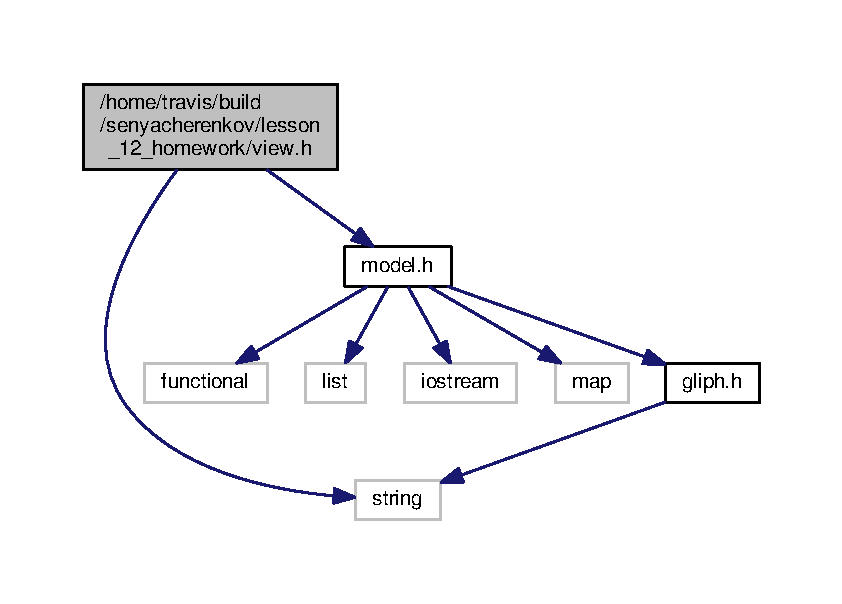
\includegraphics[width=350pt]{view_8h__incl}
\end{center}
\end{figure}
This graph shows which files directly or indirectly include this file\-:
\nopagebreak
\begin{figure}[H]
\begin{center}
\leavevmode
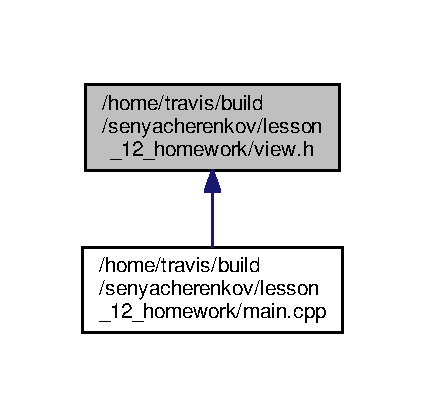
\includegraphics[width=204pt]{view_8h__dep__incl}
\end{center}
\end{figure}
\subsection*{Classes}
\begin{DoxyCompactItemize}
\item 
class \hyperlink{classView}{View}
\end{DoxyCompactItemize}

%--- End generated contents ---

% Index
\newpage
\phantomsection
\addcontentsline{toc}{chapter}{Index}
\printindex

\end{document}
